\documentclass[border=5pt]{standalone}
\usepackage[dvipsnames]{xcolor}
\usepackage{tikz}
\usetikzlibrary{arrows.meta,positioning,calc,fit,backgrounds,decorations.pathreplacing}
\usepackage{amssymb}

\definecolor{cL1}{HTML}{1565C0}
\definecolor{cL2}{HTML}{E65100}
\definecolor{cL3}{HTML}{2E7D32}
\definecolor{cL4}{HTML}{00695C}
\definecolor{cAtk}{HTML}{C62828}
\definecolor{cBelief}{HTML}{6A1B9A}
\definecolor{cMetric}{HTML}{37474F}
\definecolor{cReal}{HTML}{1B5E20}

\begin{document}
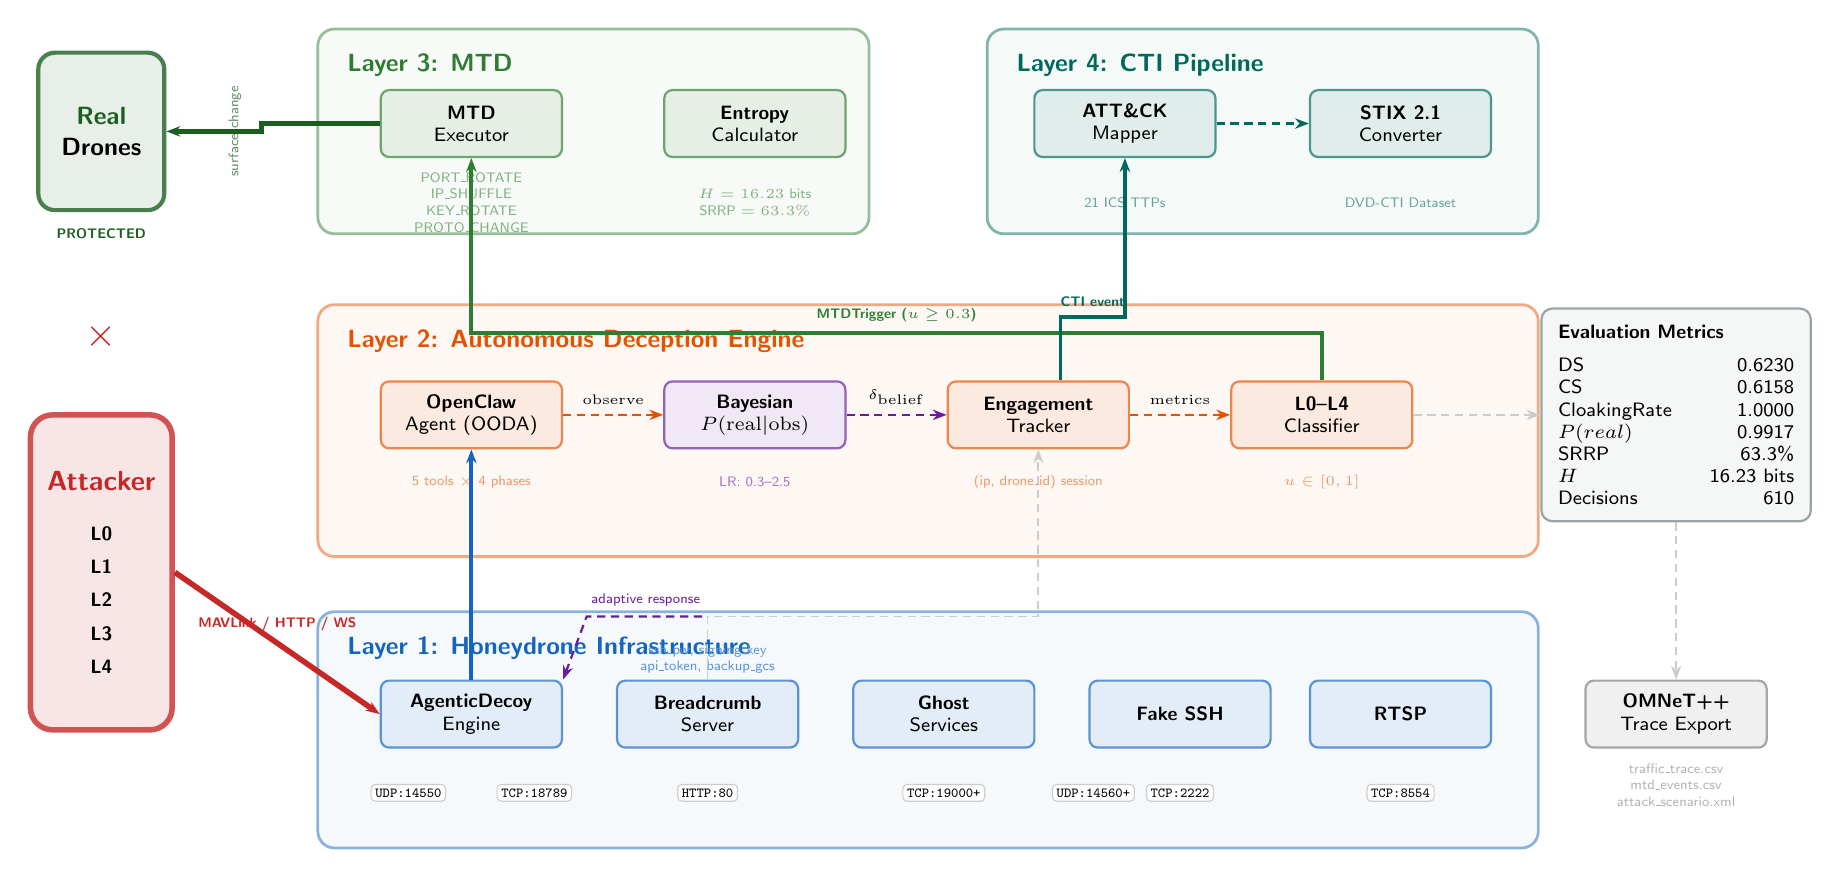
\begin{tikzpicture}[
  >={Stealth[length=5pt]},
  font=\sffamily,
  layerbg/.style={
    rectangle, rounded corners=6pt, draw=#1!50, fill=#1!4,
    line width=1pt
  },
  comp/.style={
    rectangle, rounded corners=3pt, draw=#1!70, fill=#1!12,
    line width=0.8pt, minimum width=2.3cm, minimum height=0.85cm,
    align=center, font=\sffamily\scriptsize
  },
  portlabel/.style={
    rectangle, rounded corners=1.5pt, draw=gray!40, fill=white,
    font=\ttfamily\tiny, inner sep=1.5pt
  },
  flowmain/.style={->, line width=1.4pt, draw=#1},
  flowsub/.style={->, line width=0.6pt, draw=gray!40, densely dashed},
  flowdata/.style={->, line width=0.8pt, draw=#1, densely dashed},
]

% ════════════════════════════════════════════════════
% LAYER 1 — Honeydrone Infrastructure
% ════════════════════════════════════════════════════
\node[layerbg=cL1, minimum width=15.5cm, minimum height=3.0cm] (bg1) at (8, 0) {};
\node[font=\sffamily\bfseries\small, text=cL1, anchor=north west] at (0.5, 1.3) {Layer 1: Honeydrone Infrastructure};

\node[comp=cL1] (engine) at (2.2, 0.2) {\textbf{AgenticDecoy}\\Engine};
\node[comp=cL1] (bread)  at (5.2, 0.2) {\textbf{Breadcrumb}\\Server};
\node[comp=cL1] (ghost)  at (8.2, 0.2) {\textbf{Ghost}\\Services};
\node[comp=cL1] (fssh)   at (11.2, 0.2) {\textbf{Fake SSH}};
\node[comp=cL1] (rtsp)   at (14.0, 0.2) {\textbf{RTSP}};

% Ports row
\node[portlabel] at (1.4, -0.8) {UDP:14550};
\node[portlabel] at (3.0, -0.8) {TCP:18789};
\node[portlabel] at (5.2, -0.8) {HTTP:80};
\node[portlabel] at (8.2, -0.8) {TCP:19000+};
\node[portlabel] at (10.1, -0.8) {UDP:14560+};
\node[portlabel] at (11.2, -0.8) {TCP:2222};
\node[portlabel] at (14.0, -0.8) {TCP:8554};

% Breadcrumb detail
\node[font=\sffamily\tiny, text=cL1!70, align=center] at (5.2, 0.9) {ssh\_pw, signing\_key\\api\_token, backup\_gcs};

% ════════════════════════════════════════════════════
% LAYER 2 — Autonomous Deception Engine
% ════════════════════════════════════════════════════
\node[layerbg=cL2, minimum width=15.5cm, minimum height=3.2cm] (bg2) at (8, 3.8) {};
\node[font=\sffamily\bfseries\small, text=cL2, anchor=north west] at (0.5, 5.2) {Layer 2: Autonomous Deception Engine};

\node[comp=cL2] (ooda) at (2.2, 4.0) {\textbf{OpenClaw}\\Agent (OODA)};
\node[rectangle, rounded corners=3pt, draw=cBelief!70, fill=cBelief!10,
      line width=0.8pt, minimum width=2.3cm, minimum height=0.85cm,
      align=center, font=\sffamily\scriptsize]
  (belief) at (5.8, 4.0) {\textbf{Bayesian}\\$P(\mathrm{real}|\mathrm{obs})$};
\node[comp=cL2] (track) at (9.4, 4.0) {\textbf{Engagement}\\Tracker};
\node[comp=cL2] (class) at (13.0, 4.0) {\textbf{L0--L4}\\Classifier};

% Sub-labels
\node[font=\sffamily\tiny, text=cL2!60] at (2.2, 3.15) {5 tools $\times$ 4 phases};
\node[font=\sffamily\tiny, text=cBelief!60] at (5.8, 3.15) {LR: 0.3--2.5};
\node[font=\sffamily\tiny, text=cL2!60] at (9.4, 3.15) {(ip, drone\_id) session};
\node[font=\sffamily\tiny, text=cL2!60] at (13.0, 3.15) {$u \in [0,1]$};

% Internal flows
\draw[flowdata=cL2] (ooda) -- node[above, font=\tiny] {observe} (belief);
\draw[flowdata=cBelief] (belief) -- node[above, font=\tiny] {$\delta_\mathrm{belief}$} (track);
\draw[flowdata=cL2] (track) -- node[above, font=\tiny] {metrics} (class);

% L1 → L2
\draw[flowmain=cL1] (engine.north) -- (ooda.south);
\draw[flowsub] (bread.north) -- ++(0,0.8) -| (track);

% Belief → L1 feedback
\draw[flowdata=cBelief, <-] (engine.north east) -- ++(0.3,0.8) -- ++(1.5,0)
  node[above, midway, font=\sffamily\tiny, text=cBelief] {adaptive response};

% ════════════════════════════════════════════════════
% LAYER 3 — MTD (top-left)
% ════════════════════════════════════════════════════
\node[layerbg=cL3, minimum width=7cm, minimum height=2.6cm] (bg3) at (3.75, 7.6) {};
\node[font=\sffamily\bfseries\small, text=cL3, anchor=north west] at (0.5, 8.7) {Layer 3: MTD};

\node[comp=cL3] (exec) at (2.2, 7.7) {\textbf{MTD}\\Executor};
\node[comp=cL3] (entr) at (5.8, 7.7) {\textbf{Entropy}\\Calculator};

\node[font=\sffamily\tiny, text=cL3!60, align=center] at (2.2, 6.7) {PORT\_ROTATE\\IP\_SHUFFLE\\KEY\_ROTATE\\PROTO\_CHANGE};
\node[font=\sffamily\tiny, text=cL3!60, align=center] at (5.8, 6.7) {$H=16.23$ bits\\SRRP $=63.3\%$};

% L2 → L3
\draw[flowmain=cL3] (class.north) -- ++(0, 0.6) -| node[near start, above, font=\sffamily\tiny\bfseries, text=cL3] {MTDTrigger ($u \geq 0.3$)} (exec.south);

% ════════════════════════════════════════════════════
% LAYER 4 — CTI Pipeline (top-right)
% ════════════════════════════════════════════════════
\node[layerbg=cL4, minimum width=7cm, minimum height=2.6cm] (bg4) at (12.25, 7.6) {};
\node[font=\sffamily\bfseries\small, text=cL4, anchor=north west] at (9.0, 8.7) {Layer 4: CTI Pipeline};

\node[comp=cL4] (mapper) at (10.5, 7.7) {\textbf{ATT\&CK}\\Mapper};
\node[comp=cL4] (stix)   at (14.0, 7.7) {\textbf{STIX 2.1}\\Converter};

\node[font=\sffamily\tiny, text=cL4!60] at (10.5, 6.7) {21 ICS TTPs};
\node[font=\sffamily\tiny, text=cL4!60] at (14.0, 6.7) {DVD-CTI Dataset};

\draw[flowdata=cL4] (mapper) -- (stix);

% L2 → L4
\draw[flowmain=cL4] ([xshift=8pt]track.north) -- ++(0, 0.8) -| node[near start, above, font=\sffamily\tiny\bfseries, text=cL4] {CTI event} (mapper.south);

% ════════════════════════════════════════════════════
% ATTACKER (left)
% ════════════════════════════════════════════════════
\node[rectangle, rounded corners=8pt, draw=cAtk!80, fill=cAtk!12,
      line width=2pt, minimum width=1.8cm, minimum height=4.0cm,
      align=center, font=\sffamily\bfseries]
  (atk) at (-2.5, 2) {\textcolor{cAtk}{Attacker}\\[6pt]
    {\scriptsize L0}\\{\scriptsize L1}\\{\scriptsize L2}\\{\scriptsize L3}\\{\scriptsize L4}};

\draw[flowmain=cAtk, line width=2pt] (atk.east) --
  node[above, font=\sffamily\tiny\bfseries, text=cAtk] {MAVLink / HTTP / WS}
  (engine.west);

% ════════════════════════════════════════════════════
% REAL DRONES (far left, protected)
% ════════════════════════════════════════════════════
\node[rectangle, rounded corners=6pt, draw=cReal!80, fill=cReal!10,
      line width=1.5pt, minimum width=1.6cm, minimum height=2.0cm,
      align=center, font=\sffamily\bfseries\small]
  (real) at (-2.5, 7.6) {\textcolor{cReal}{Real}\\Drones};
\node[font=\sffamily\tiny\bfseries, text=cReal] at (-2.5, 6.3) {PROTECTED};

\draw[flowmain=cReal, line width=2pt] (exec.west) -- ++(-1.5,0) |- (real.east);
\node[font=\sffamily\tiny, text=cReal!70, rotate=90, anchor=south] at (-0.6, 7.6) {surface change};

% X mark — attacker cannot reach real drones
\node[font=\bfseries\Large, text=cAtk] at (-2.5, 5.0) {$\times$};

% ════════════════════════════════════════════════════
% METRICS (far right)
% ════════════════════════════════════════════════════
\node[rectangle, rounded corners=4pt, draw=cMetric!50, fill=cMetric!5,
      line width=0.8pt, align=left, font=\sffamily\scriptsize,
      text width=3.0cm, inner sep=6pt]
  (met) at (17.5, 4.0) {
    \textbf{Evaluation Metrics}\\[4pt]
    DS\hfill 0.6230\\
    CS\hfill 0.6158\\
    CloakingRate\hfill 1.0000\\
    $P(\text{real})$\hfill 0.9917\\
    SRRP\hfill 63.3\%\\
    $H$\hfill 16.23 bits\\
    Decisions\hfill 610
  };

\draw[flowsub] (class.east) -- ++(0.5,0) |- (met.west);

% OMNeT++
\node[comp=gray, font=\sffamily\scriptsize] (omnet) at (17.5, 0.2) {\textbf{OMNeT++}\\Trace Export};
\draw[flowsub] (met.south) -- (omnet.north);
\node[font=\sffamily\tiny, text=gray!60, align=center] at (17.5, -0.7) {traffic\_trace.csv\\mtd\_events.csv\\attack\_scenario.xml};

\end{tikzpicture}
\end{document}
